% =====================================================================
%  Függvények, exponenciális, logaritmus, trigonometria
%
%  JAVÍTOTT FORRÁSHIBÁK
%   [p3] f(2) = 2^3 = 2   ->  8
%   [p3] negyedfokú polinom feltétele: c != 0  ->  a != 0
%   [p4] a 10^x értékkészleténél ÉT = R^+  ->  ÉK = R^+
%   [p5] a log_2 x grafikonjánál ÉT: R  ->  ÉT: R^+
%   [p7] az egységkörön (sin α, cos α)  ->  (cos α, sin α)
%   [p9] sin(x + k2π) jobb oldala hiányzott  ->  = sin x
%   [p10] sin(-77π/6) eredménye 1/2  ->  -1/2
%   [p11] a linearizáló formula számlálójában sin^2 1  ->  sin^2 x
%
%  KIEGÉSZÍTÉS
%   [p2] a szigorú monotonitás definíciója
%   [p3] harmadfokú polinom feltétele: a != 0
%   [p4] az exponenciális függvény értelmezési tartománya: ÉT = R
%   [p7] egy tagmondat arról, hogy tetszőleges α esetén cos α és sin α
%        az egységkör megfelelő pontjának koordinátái
%   [p9] a tg π szerinti periodicitása, a p8-beli tg(α + 180°) = tg α
%        alapján
% =====================================================================

\documentclass[11pt]{article}
\input{preamble}
\input{macros}

\begin{document}
\titleblock{Függvények, exponenciális, logaritmus, trigonometria}

% ===================================================================
\section{Függvények}

% [p1]
\begin{defbox}
\begin{definition}[Függvény]
Legyen $A$ és $B$ két halmaz. Ha $A$ minden eleméhez egy $B$-beli elemet rendelünk, akkor egy $A$-ból $B$-be képező \emph{függvényt} definiálunk.
\end{definition}
\end{defbox}

\begin{notefig}{Az $A$-ból $B$-be képező $f$ függvény.}
\begin{tikzpicture}[scale=1.0,>=Stealth]
\draw[thick] (0,0) ellipse (1.15 and 0.85);
\node[below] at (0,-0.95) {$A$};
\draw[thick] (3.5,-0.25) ellipse (0.85 and 0.62);
\node[below] at (3.5,-0.95) {$B$};
\fill (-0.1,0.1) circle (1.3pt) node[below,font=\footnotesize] {$a$};
\fill (3.45,-0.2) circle (1.3pt) node[below,font=\footnotesize] {$b$};
\draw[thick,accent,->] (-0.1,0.25) to[out=60,in=120] (3.4,-0.05);
\node[accent,above] at (1.7,0.95) {$f$};
\node[right,font=\footnotesize] at (4.7,-0.25) {$b=f(a)$};
\end{tikzpicture}
\end{notefig}

\begin{defbox}
\begin{definition}[Értelmezési tartomány, értékkészlet]
Az $A$ halmaz az $f$ függvény \emph{értelmezési tartománya}. Jelölés: $D_f$ v.\ $\ET$. Azon $B$-beli elemek összessége, ami fellép képeltként, az $f$ függvény \emph{értékkészlete}. Jelölés: $R_f$ v.\ $\EK$. Tehát
\[
\EK=\bigl\{\,b:\ \text{létezik } a\in A, \text{ hogy } b=f(a)\,\bigr\}.
\]
\end{definition}
\end{defbox}
Mi olyan függvényekkel foglalkozunk, ahol az $\ET$ a valós számok vagy annak részhalmaza. Ezek a \emph{valós függvények}.

% ===================================================================
\section{Polinomok}

% [p1]
\begin{defbox}
\begin{definition}[Elsőfokú polinom]
\[
f(x)=ax+b,\qquad a\neq 0 \quad \text{(egyenes)}.
\]
\end{definition}
\end{defbox}

\begin{exbox}
\begin{example}
$f(x)=2x+3$.
\end{example}
\end{exbox}
\begin{solution}
$\ET=\R$ és $\EK=\R$.

\begin{notefig}{Az $f(x)=2x+3$ függvény grafikonja.}
\begin{tikzpicture}
\begin{axis}[funcplot, xmin=-3.2, xmax=2.2, ymin=-3.4, ymax=6.4,
  xtick={-2,-1,1,2}, ytick={3}]
\addplot[domain=-3:1.6]{2*x+3};
\end{axis}
\end{tikzpicture}
\end{notefig}
\end{solution}

% [p2]
\begin{defbox}
\begin{definition}[Másodfokú polinom]
\[
f(x)=ax^{2}+bx+c,\qquad a\neq 0 \quad \text{(parabola)},
\]
és $\ET=\R$.
\end{definition}
\end{defbox}

\begin{exbox}
\begin{example}
$f(x)=x^{2}$.
\end{example}
\end{exbox}
\begin{solution}
$\EK=\{y:\ y\ge 0\}$.

\begin{notefig}{Az $f(x)=x^{2}$ függvény grafikonja.}
\begin{tikzpicture}
\begin{axis}[funcplot, xmin=-2.6, xmax=2.6, ymin=-1.0, ymax=5.0,
  xtick={-2,-1,1,2}, ytick={1,2,3,4}]
\addplot[domain=-2.2:2.2]{x^2};
\end{axis}
\end{tikzpicture}
\end{notefig}
\end{solution}

\begin{exbox}
\begin{example}
$f(x)=x^{2}+5x+6$.
\end{example}
\end{exbox}
\begin{solution}
A zérushelyek az $x^{2}+5x+6=0$ egyenletből
\[
x_{1,2}=\frac{-5\pm\sqrt{25-24}}{2}=
\begin{cases}
-2,\\
-3 .
\end{cases}
\]
$x=-2,5$-ben veszi fel a legkisebb értékét:
\[
f(-2,5)=(-2,5)^{2}+5\cdot(-2,5)+6=-\frac{1}{4},
\]
tehát $\EK=\left\{y:\ y\ge -\tfrac{1}{4}\right\}$.

\begin{notefig}{Az $f(x)=x^{2}+5x+6$ függvény grafikonja.}
\begin{tikzpicture}
\begin{axis}[funcplot, xmin=-4.6, xmax=1.6, ymin=-1.6, ymax=4.4,
  xtick={-3,-2.5,-2,-1,1}, xticklabels={$-3$,$-2{,}5$,$-2$,,},
  ytick={1,2,3}]
\addplot[domain=-4.2:-0.8]{x^2+5*x+6};
\addplot[only marks,mark=*,mark size=1.4pt,thmaccent]
  coordinates {(-3,0) (-2,0) (-2.5,-0.25)};
\end{axis}
\end{tikzpicture}
\end{notefig}
\end{solution}

\begin{defbox}
\begin{definition}[Monotonitás]
Az $f(x)$ függvény \emph{monoton nő} (\emph{csökken}) az $I$ intervallumban, ha minden $x_{1}<x_{2}$, $x_{1}, x_{2}\in I$ esetén
\[
f(x_{1})\le f(x_{2})\qquad \bigl(f(x_{1})\ge f(x_{2})\bigr).
\]
\end{definition}
\end{defbox}

\begin{defbox}
\begin{definition}[Szigorú monotonitás]
Az $f(x)$ függvény \emph{szigorúan monoton nő} (\emph{csökken}) az $I$ intervallumban, ha minden $x_{1}<x_{2}$, $x_{1}, x_{2}\in I$ esetén
\[
f(x_{1})<f(x_{2})\qquad \bigl(f(x_{1})>f(x_{2})\bigr).
\]
\end{definition}
\end{defbox}

\begin{defbox}
\begin{definition}[Korlátosság]
Az $f(x)$ \emph{alulról} (\emph{felülről}) \emph{korlátos} függvény, ha létezik $K$, hogy
\[
f(x)\ge K\qquad \bigl(f(x)\le K\bigr)
\]
minden $x\in D_{f}$ esetén. Az $f(x)$ függvény \emph{korlátos}, ha felülről és alulról is korlátos.
\end{definition}
\end{defbox}

\begin{exbox}
\begin{example}
$f(x)=-2x^{2}+x+1$.
\end{example}
\end{exbox}
\begin{solution}
A zérushelyek
\[
x_{1,2}=\frac{-1\pm\sqrt{1+8}}{-4}=
\begin{cases}
1,\\
-\tfrac{1}{2} .
\end{cases}
\]
A szélsőérték
\[
f\!\left(\frac{1}{4}\right)=-2\left(\frac{1}{4}\right)^{2}+\frac{1}{4}+1=\frac{9}{8},
\]
tehát $\EK=\left\{y:\ y\le \tfrac{9}{8}\right\}$, és a függvény felülről korlátos. A
$\left]-\infty, \tfrac{1}{4}\right[$ intervallumban monoton nő, a
$\left]\tfrac{1}{4}, +\infty\right[$ intervallumban monoton csökken.

\begin{notefig}{Az $f(x)=-2x^{2}+x+1$ függvény grafikonja.}
\begin{tikzpicture}
\begin{axis}[funcplot, xmin=-1.6, xmax=1.9, ymin=-2.2, ymax=1.9,
  xtick={-0.5,0.25,1}, xticklabels={$-\frac12$,$\frac14$,$1$},
  ytick={1}]
\addplot[domain=-1.1:1.5]{-2*x^2+x+1};
\addplot[only marks,mark=*,mark size=1.4pt,thmaccent]
  coordinates {(-0.5,0) (1,0) (0.25,1.125)};
\end{axis}
\end{tikzpicture}
\end{notefig}
\end{solution}

% [p3]
\begin{defbox}
\begin{definition}[Harmadfokú polinom]
\[
f(x)=ax^{3}+bx^{2}+cx+d,\qquad a, b, c, d\in\R,\ a\neq 0,
\]
és $\ET=\R$.
\end{definition}
\end{defbox}

\begin{exbox}
\begin{example}
$f(x)=x^{3}$.
\end{example}
\end{exbox}
\begin{solution}
\[
f(0)=0^{3}=0,\quad f(1)=1^{3}=1,\quad f(2)=2^{3}=8,\quad
f(-1)=(-1)^{3}=-1,\quad f(-2)=(-2)^{3}=-8 .
\]
A függvény monoton nő és nem korlátos.

\begin{notefig}{Az $f(x)=x^{3}$ függvény grafikonja.}
\begin{tikzpicture}
\begin{axis}[funcplot, xmin=-2.6, xmax=2.6, ymin=-9.0, ymax=9.0,
  xtick={-2,-1,1,2}, ytick={-8,-1,1,8}]
\addplot[domain=-2.1:2.1]{x^3};
\end{axis}
\end{tikzpicture}
\end{notefig}
\end{solution}

\begin{exbox}
\begin{example}
$f(x)=x^{3}-x$.
\end{example}
\end{exbox}
\begin{solution}
A zérushelyek
\[
x^{3}-x=0,\qquad x(x^{2}-1)=0,\qquad x=0,\ \pm 1 .
\]
A függvény nem korlátos és $\EK=\R$. Később megmutatjuk, hogy a
$\left]-\infty, -\tfrac{1}{\sqrt{3}}\right[$ és a
$\left]\tfrac{1}{\sqrt{3}}, +\infty\right[$ intervallumban monoton nő, a
$\left]-\tfrac{1}{\sqrt{3}}, \tfrac{1}{\sqrt{3}}\right[$ intervallumban monoton csökken.

\begin{notefig}{Az $f(x)=x^{3}-x$ függvény grafikonja.}
\begin{tikzpicture}
\begin{axis}[funcplot, xmin=-1.9, xmax=1.9, ymin=-1.9, ymax=1.9,
  xtick={-1,1}, ytick={-1,1}]
\addplot[domain=-1.6:1.6]{x^3-x};
\addplot[only marks,mark=*,mark size=1.4pt,thmaccent]
  coordinates {(-1,0) (0,0) (1,0)};
\end{axis}
\end{tikzpicture}
\end{notefig}
\end{solution}

\begin{defbox}
\begin{definition}[Negyedfokú polinom]
\[
f(x)=ax^{4}+bx^{3}+cx^{2}+dx+e,\qquad a, b, c, d, e\in\R,\ a\neq 0,
\]
és $\ET=\R$.
\end{definition}
\end{defbox}

\begin{exbox}
\begin{example}
$f(x)=x^{4}$.
\end{example}
\end{exbox}
\begin{solution}
$\EK=\{y:\ y\ge 0\}$.

\begin{notefig}{Az $f(x)=x^{4}$ függvény grafikonja.}
\begin{tikzpicture}
\begin{axis}[funcplot, xmin=-2.4, xmax=2.4, ymin=-1.2, ymax=6.0,
  xtick={-2,-1,1,2}, ytick={1,2,3,4,5}]
\addplot[domain=-1.55:1.55]{x^4};
\end{axis}
\end{tikzpicture}
\end{notefig}
\end{solution}

% [p4]
\begin{defbox}
\begin{definition}[$n$-edfokú polinom]
\[
a_{n}x^{n}+a_{n-1}x^{n-1}+a_{n-2}x^{n-2}+\dots+a_{1}x+a_{0},
\qquad a_{i}\in\R,\ a_{n}\neq 0 .
\]
\end{definition}
\end{defbox}

% ===================================================================
\section{Páros és páratlan függvények}

% [p4]
\begin{defbox}
\begin{definition}[Páros függvény]
Az $f(x)$ függvény \emph{páros}, ha grafikonja az $y$ tengelyre szimmetrikus, azaz
\[
f(x)=f(-x).
\]
\end{definition}
\end{defbox}
Pl.\ $f(x)=x^{2}$, $x^{4}$.

\begin{defbox}
\begin{definition}[Páratlan függvény]
Az $f(x)$ függvény \emph{páratlan}, ha grafikonja az origóra szimmetrikus, azaz
\[
f(-x)=-f(x).
\]
\end{definition}
\end{defbox}
Pl.\ $f(x)=x$, $x^{3}$, $x^{3}-x$.

% ===================================================================
\section{Exponenciális függvények}

% [p4]
\begin{defbox}
\begin{definition}[Exponenciális függvény]
Legyen $a>0$. Az
\[
f(x)=a^{x}
\]
függvényt \emph{exponenciális függvénynek} hívjuk. Ekkor $\ET=\R$.
\end{definition}
\end{defbox}

\begin{exbox}
\begin{example}
$f(x)=10^{x}$.
\end{example}
\end{exbox}
\begin{solution}
\[
f(0)=10^{0}=1,\quad f(1)=10^{1}=10,\quad f(2)=10^{2}=100,\quad f(3)=10^{3}=1000,
\]
\[
f(-1)=10^{-1}=\frac{1}{10}=0,1,\qquad f(-2)=10^{-2}=\frac{1}{100}=0,01 .
\]
$\EK=\R^{+}=\{y:\ y>0\}$, és a függvény monoton nő.

\begin{notefig}{Az $f(x)=10^{x}$ függvény grafikonja.}
\begin{tikzpicture}
\begin{axis}[funcplot, xmin=-2.6, xmax=2.0, ymin=-1.6, ymax=11.5,
  xtick={-2,-1,1,2}, ytick={1,10}]
\addplot[domain=-2.3:1.04]{10^x};
\end{axis}
\end{tikzpicture}
\end{notefig}
\end{solution}

\begin{exbox}
\begin{example}
$f(x)=\left(\tfrac{1}{2}\right)^{x}$.
\end{example}
\end{exbox}
\begin{solution}
\[
f(0)=\left(\frac{1}{2}\right)^{0}=1,\quad
f(1)=\left(\frac{1}{2}\right)^{1}=\frac{1}{2}=0,5,\quad
f(2)=\left(\frac{1}{2}\right)^{2}=\frac{1}{4}=0,25,
\]
\[
f(3)=\left(\frac{1}{2}\right)^{3}=\frac{1}{8}=0,125,\qquad
f(-1)=\left(\frac{1}{2}\right)^{-1}=2,
\]
\[
f(-2)=\left(\frac{1}{2}\right)^{-2}=\left(2^{-1}\right)^{-2}=2^{2}=4,\qquad
f(-3)=\left(\frac{1}{2}\right)^{-3}=2^{3}=8 .
\]
A függvény monoton csökken, és $\EK=\R^{+}$.

\begin{notefig}{Az $f(x)=\left(\tfrac{1}{2}\right)^{x}$ függvény grafikonja.}
\begin{tikzpicture}
\begin{axis}[funcplot, xmin=-2.6, xmax=3.6, ymin=-1.2, ymax=5.2,
  xtick={-2,-1,1,2,3}, ytick={1,2,3,4}]
\addplot[domain=-2.05:3.3]{2^(-x)};
\end{axis}
\end{tikzpicture}
\end{notefig}
\end{solution}

Általában:

\begin{notefig}{Az $a^{x}$ függvény alakja $a>1$, illetve $0<a<1$ esetén.}
\begin{tikzpicture}
\begin{axis}[smallplot, title={\footnotesize $a>1$, monoton nő},
  xmin=-2.4, xmax=2.4, ymin=-0.8, ymax=4.2, xtick=\empty, ytick={1}]
\addplot[domain=-2.1:2.05]{2^x};
\end{axis}
\end{tikzpicture}\hspace{0.6em}
\begin{tikzpicture}
\begin{axis}[smallplot, title={\footnotesize $0<a<1$, monoton csökken},
  xmin=-2.4, xmax=2.4, ymin=-0.8, ymax=4.2, xtick=\empty, ytick={1}]
\addplot[domain=-2.05:2.1]{2^(-x)};
\end{axis}
\end{tikzpicture}
\end{notefig}

% ===================================================================
\section{Logaritmus}

% [p5]
\begin{defbox}
\begin{definition}[Logaritmus]
Legyen $a>0$, $a\neq 1$, $b>0$. Ekkor egyetlen olyan $y$ valós szám van, amire $a^{y}=b$, és ezt
\[
y=\log_{a} b
\]
jelöli ($a$ alapú logaritmus $b$).
\end{definition}
\end{defbox}

\begin{exbox}
\begin{example}
Számítsuk ki a következő logaritmusokat.
\end{example}
\end{exbox}
\begin{solution}
$2^{y}=8 \Rightarrow y=3$, azaz $\log_{2}8=3$. Továbbá
\[
\log_{10}10000=4,\quad \text{mert}\quad 10^{4}=10000,
\]
\[
\log_{3}9=2,\quad \text{mert}\quad 3^{2}=9,
\]
\[
\log_{1/2}8=-3,\quad \text{mert}\quad
\left(\frac{1}{2}\right)^{-3}=\left(2^{-1}\right)^{-3}=2^{3}=8 .
\]
\end{solution}

Tudjuk, hogy $a>0$, $a\neq 1$ esetén minden $x>0$ esetén létezik $y$ valós szám, hogy $x=a^{y}$. Ekkor $y=\log_{a}x$. Így egy olyan függvényt értelmezhetünk, ahol $\ET=\R^{+}$.

\begin{exbox}
\begin{example}
$a=2$, $y=\log_{2}x$.
\end{example}
\end{exbox}
\begin{solution}
\begin{align*}
x&=1: & \log_{2}1&=0, && \text{mert } 2^{0}=1,\\
x&=2: & \log_{2}2&=1, && \text{mert } 2^{1}=2,\\
x&=4: & \log_{2}4&=2, && \text{mert } 2^{2}=4,\\
x&=8: & \log_{2}8&=3, && \text{mert } 2^{3}=8,\\
x&=\tfrac{1}{2}: & \log_{2}\tfrac{1}{2}&=-1, && \text{mert } 2^{-1}=\tfrac{1}{2},\\
x&=\tfrac{1}{4}: & \log_{2}\tfrac{1}{4}&=-2, && \text{mert } 2^{-2}=\tfrac{1}{4}.
\end{align*}
$\ET=\R^{+}$, a függvény monoton nő, és $\EK=\R$.

\begin{notefig}{A $\log_{2}x$ függvény grafikonja.}
\begin{tikzpicture}
\begin{axis}[funcplot, xmin=-0.6, xmax=9.2, ymin=-2.8, ymax=3.4,
  xtick={0.25,0.5,1,2,3,4,5,6,7,8},
  xticklabels={,,$1$,$2$,$3$,$4$,$5$,$6$,$7$,$8$},
  ytick={-2,-1,1,2,3}]
\addplot[domain=0.13:8.6]{ln(x)/ln(2)};
\addplot[only marks,mark=*,mark size=1.2pt,thmaccent]
  coordinates {(1,0) (2,1) (4,2) (8,3) (0.5,-1) (0.25,-2)};
\end{axis}
\end{tikzpicture}
\end{notefig}
\end{solution}

% [p6]
\begin{exbox}
\begin{example}
$a=\tfrac{1}{3}$.
\end{example}
\end{exbox}
\begin{solution}
\begin{align*}
\log_{1/3}1&=0, && \left(\tfrac{1}{3}\right)^{0}=1, &
\log_{1/3}\tfrac{1}{3}&=1, && \left(\tfrac{1}{3}\right)^{1}=\tfrac{1}{3},\\
\log_{1/3}3&=-1, && \left(\tfrac{1}{3}\right)^{-1}=3, &
\log_{1/3}\tfrac{1}{9}&=2, && \left(\tfrac{1}{3}\right)^{2}=\tfrac{1}{9},\\
\log_{1/3}9&=-2, && \left(\tfrac{1}{3}\right)^{-2}=9 . & & & &
\end{align*}
$\ET=\R^{+}$, a függvény monoton csökken, és $\EK=\R$.

\begin{notefig}{A $\log_{1/3}x$ függvény grafikonja.}
\begin{tikzpicture}
\begin{axis}[funcplot, xmin=-0.6, xmax=9.2, ymin=-2.8, ymax=3.4,
  xtick={1,3,9}, ytick={-2,-1,1,2,3}]
\addplot[domain=0.09:8.9]{ln(x)/ln(1/3)};
\addplot[only marks,mark=*,mark size=1.2pt,thmaccent]
  coordinates {(1,0) (3,-1) (9,-2) (0.3333,1) (0.1111,2)};
\end{axis}
\end{tikzpicture}
\end{notefig}
\end{solution}

Általában:

\begin{notefig}{A $\log_{a}x$ függvény alakja $a>1$, illetve $0<a<1$ esetén.}
\begin{tikzpicture}
\begin{axis}[smallplot, title={\footnotesize $a>1$, nő},
  xmin=-0.5, xmax=4.4, ymin=-2.6, ymax=2.6, xtick={1}, ytick=\empty]
\addplot[domain=0.18:4.2]{ln(x)/ln(2)};
\end{axis}
\end{tikzpicture}\hspace{0.6em}
\begin{tikzpicture}
\begin{axis}[smallplot, title={\footnotesize $0<a<1$, csökken},
  xmin=-0.5, xmax=4.4, ymin=-2.6, ymax=2.6, xtick={1}, ytick=\empty]
\addplot[domain=0.18:4.2]{ln(x)/ln(1/2)};
\end{axis}
\end{tikzpicture}
\end{notefig}

\begin{thmbox}
\begin{theorem}[A logaritmus tulajdonságai]
Legyen $a>0$, $a\neq 1$.
\begin{enumerate}[label=\arabic*.]
\item Ha $u, v>0$, akkor $\log_{a}(uv)=\log_{a}u+\log_{a}v$.
\item Ha $u, v>0$, akkor $\log_{a}\dfrac{u}{v}=\log_{a}u-\log_{a}v$.
\item Ha $u>0$ és $w\in\R$, akkor $\log_{a}u^{w}=w\log_{a}u$.
\end{enumerate}
\end{theorem}
\end{thmbox}
\begin{proof}
1. Egyrészt $uv=a^{\log_{a}(uv)}$, másrészt
\[
uv=a^{\log_{a}u}\cdot a^{\log_{a}v}=a^{\log_{a}u+\log_{a}v},
\]
és mivel $a^{x}$ kölcsönösen egyértelmű, a két kitevő megegyezik, tehát
\[
\log_{a}(uv)=\log_{a}u+\log_{a}v .
\]
2. Hasonlóan adódik.

3. Egyrészt $u^{w}=a^{\log_{a}(u^{w})}$, másrészt
\[
u^{w}=\left(a^{\log_{a}u}\right)^{w}=a^{w\log_{a}u},
\]
ahonnan $\log_{a}u^{w}=w\log_{a}u$.
\end{proof}

% ===================================================================
\section{Trigonometrikus függvények}

% [p7]
\begin{defbox}
\begin{definition}[Szögfüggvények derékszögű háromszögben]
Legyen $0<\alpha<90^{\circ}$. Ekkor
\[
\sin\alpha=\frac{a}{c},\qquad \cos\alpha=\frac{b}{c},
\]
\[
\tg\alpha=\frac{a}{b}=\frac{\sin\alpha}{\cos\alpha},\qquad
\ctg\alpha=\frac{b}{a}=\frac{\cos\alpha}{\sin\alpha}=\frac{1}{\tg\alpha}.
\]
\end{definition}
\end{defbox}

\begin{notefig}{A derékszögű háromszög jelölései.}
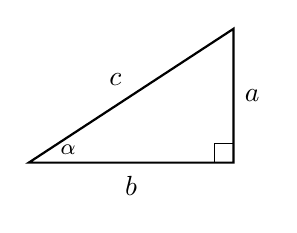
\begin{tikzpicture}[scale=1.0]
\coordinate (A) at (0,0);
\coordinate (C) at (2.6,0);
\coordinate (B) at (2.6,1.7);
\draw[thick] (A) -- (C) -- (B) -- cycle;
\draw (2.6,0.24) -- (2.36,0.24) -- (2.36,0);
\node[below] at (1.3,-0.05) {$b$};
\node[right] at (2.62,0.85) {$a$};
\node[above left] at (1.3,0.85) {$c$};
\node[right,font=\footnotesize] at (0.28,0.16) {$\alpha$};
\end{tikzpicture}
\end{notefig}

\noindent Nevezetes szögfüggvényértékek:
\begin{center}
\renewcommand{\arraystretch}{1.7}
\begin{tabular}{c|ccc}
\hline
$\alpha$ & $30^{\circ}$ & $45^{\circ}$ & $60^{\circ}$\\
\hline
$\sin\alpha$ & $\frac{1}{2}$ & $\frac{\sqrt{2}}{2}$ & $\frac{\sqrt{3}}{2}$\\
$\cos\alpha$ & $\frac{\sqrt{3}}{2}$ & $\frac{\sqrt{2}}{2}$ & $\frac{1}{2}$\\
$\tg\alpha$ & $\frac{1}{\sqrt{3}}$ & $1$ & $\sqrt{3}$\\
\hline
\end{tabular}
\end{center}

Másképp:

\begin{notefig}{Az egységkör pontja az $\alpha$ szöghöz. A beírt derékszögű
háromszög átfogója $1$, ezért a befogók hossza épp $\cos\alpha$ és $\sin\alpha$.}
\begin{tikzpicture}[scale=1.65,>=Stealth]
\draw[->] (-1.55,0) -- (1.95,0) node[below,font=\footnotesize] {};
\draw[->] (0,-1.55) -- (0,1.95);
\draw[thick] (0,0) circle (1.3);
\coordinate (O) at (0,0);
\coordinate (P) at (50:1.3);
\coordinate (Q) at ({1.3*cos(50)},0);
% a beírt derékszögű háromszög
\fill[exbg] (O) -- (Q) -- (P) -- cycle;
\draw[thick,thmaccent] (Q) -- (P);
\draw[thick,thmaccent] (O) -- (Q);
\draw[thick,accent] (O) -- (P);
\draw ({1.3*cos(50)-0.13},0) -- ({1.3*cos(50)-0.13},0.13) -- ({1.3*cos(50)},0.13);
\draw[accent] (0.34,0) arc (0:50:0.34);
\node[accent,font=\footnotesize] at (0.56,0.18) {$\alpha$};
\node[accent,font=\footnotesize,fill=white,inner sep=1pt] at (0.30,0.62) {$1$};
\node[thmaccent,font=\footnotesize,below,fill=white,inner sep=1pt]
  at ({1.3*cos(50)/2},-0.03) {$\cos\alpha$};
\node[thmaccent,font=\footnotesize,right,fill=white,inner sep=1pt]
  at ({1.3*cos(50)+0.02},0.34) {$\sin\alpha$};
\fill (P) circle (1.3pt) node[above right,font=\footnotesize] {$(\cos\alpha, \sin\alpha)$};
\node[font=\footnotesize,below,fill=white,inner sep=1pt] at (1.3,-0.05) {$1$};
\node[font=\footnotesize,below,fill=white,inner sep=1pt] at (-1.3,-0.05) {$-1$};
\node[font=\footnotesize,left,fill=white,inner sep=1pt] at (-0.05,-1.3) {$-1$};
\node[font=\footnotesize,left,fill=white,inner sep=1pt] at (-0.05,1.3) {$1$};
\end{tikzpicture}
\end{notefig}

\noindent Ez lehetőséget ad, hogy tetszőleges $\alpha$ fok esetén $\sin\alpha$-t és $\cos\alpha$-t definiáljuk: $\cos\alpha$ és $\sin\alpha$ annak a pontnak az első, illetve második koordinátája, amelybe az egységkörön a pozitív $x$ tengelytől $\alpha$ szöget bemérve jutunk.

\begin{exbox}
\begin{example}
$\alpha=135^{\circ}$.
\end{example}
\end{exbox}
\begin{solution}
A $45^{\circ}$-hoz tartozó pont $\left(\tfrac{\sqrt{2}}{2}, \tfrac{\sqrt{2}}{2}\right)$, és ennek az $y$ tengelyre vett tükörképe a $135^{\circ}$-hoz tartozó pont (szimmetria), tehát
\[
(\cos 135^{\circ}, \sin 135^{\circ})=\left(-\frac{\sqrt{2}}{2}, \frac{\sqrt{2}}{2}\right),
\]
azaz $\cos 135^{\circ}=-\tfrac{\sqrt{2}}{2}$ és $\sin 135^{\circ}=\tfrac{\sqrt{2}}{2}$.

\begin{notefig}{A $135^{\circ}$ és a $45^{\circ}$ szöghöz tartozó pont.}
\begin{tikzpicture}[scale=1.25,>=Stealth]
\draw[->] (-1.5,0) -- (1.6,0);
\draw[->] (0,-1.5) -- (0,1.6);
\draw[thick] (0,0) circle (1.2);
\draw[thick,accent] (0,0) -- (135:1.2);
\draw[thmaccent,dashed] (0,0) -- (45:1.2);
\draw[thmaccent,dashed] (135:1.2) -- (45:1.2);
\draw[accent] (0.38,0) arc (0:135:0.38);
\node[accent,font=\scriptsize] at (-0.14,0.52) {$135^{\circ}$};
\node[thmaccent,font=\scriptsize] at (0.72,0.26) {$45^{\circ}$};
\fill (135:1.2) circle (1.2pt);
\fill (45:1.2) circle (1.2pt) node[above right,font=\footnotesize]
  {$\left(\tfrac{\sqrt{2}}{2}, \tfrac{\sqrt{2}}{2}\right)$};
\node[font=\footnotesize,below] at (1.2,-0.06) {$1$};
\end{tikzpicture}
\end{notefig}
\end{solution}

\begin{exbox}
\begin{example}
$\alpha=210^{\circ}$.
\end{example}
\end{exbox}
\begin{solution}
A $30^{\circ}$-hoz tartozó pont $(\cos 30^{\circ}, \sin 30^{\circ})=\left(\tfrac{\sqrt{3}}{2}, \tfrac{1}{2}\right)$, és ennek az origóra vett tükörképe a $210^{\circ}$-hoz tartozó pont (szimmetria), tehát
\[
(\cos 210^{\circ}, \sin 210^{\circ})=\left(-\frac{\sqrt{3}}{2}, -\frac{1}{2}\right),
\]
azaz $\cos 210^{\circ}=-\tfrac{\sqrt{3}}{2}$ és $\sin 210^{\circ}=-\tfrac{1}{2}$.

\begin{notefig}{A $210^{\circ}$ és a $30^{\circ}$ szöghöz tartozó pont.}
\begin{tikzpicture}[scale=1.25,>=Stealth]
\draw[->] (-1.5,0) -- (1.6,0);
\draw[->] (0,-1.5) -- (0,1.6);
\draw[thick] (0,0) circle (1.2);
\draw[thick,accent] (0,0) -- (210:1.2);
\draw[thmaccent,dashed] (0,0) -- (30:1.2);
\draw[accent] (0.38,0) arc (0:210:0.38);
\node[accent,font=\scriptsize] at (-0.30,0.50) {$210^{\circ}$};
\node[thmaccent,font=\scriptsize] at (0.74,0.20) {$30^{\circ}$};
\fill (210:1.2) circle (1.2pt);
\fill (30:1.2) circle (1.2pt) node[above right,font=\footnotesize]
  {$\left(\tfrac{\sqrt{3}}{2}, \tfrac{1}{2}\right)$};
\node[font=\footnotesize,below] at (1.2,-0.06) {$1$};
\end{tikzpicture}
\end{notefig}
\end{solution}

% [p8]
\noindent Nevezetes szögfüggvény értékek:
\begin{center}
\renewcommand{\arraystretch}{1.7}
\begin{tabular}{c|ccccc}
\hline
$\alpha$ & $0^{\circ}$ & $90^{\circ}$ & $120^{\circ}$ & $135^{\circ}$ & $150^{\circ}$\\
\hline
$\sin\alpha$ & $0$ & $1$ & $\frac{\sqrt{3}}{2}$ & $\frac{\sqrt{2}}{2}$ & $\frac{1}{2}$\\
$\cos\alpha$ & $1$ & $0$ & $-\frac{1}{2}$ & $-\frac{\sqrt{2}}{2}$ & $-\frac{\sqrt{3}}{2}$\\
$\tg\alpha$ & $0$ & $\ast$ & $-\sqrt{3}$ & $-1$ & $-\frac{1}{\sqrt{3}}$\\
\hline
\end{tabular}
\end{center}
\noindent {\footnotesize $\ast$\ A $\tg 90^{\circ}=\dfrac{\sin 90^{\circ}}{\cos 90^{\circ}}=\dfrac{1}{0}$ érték nincs értelmezve.}

\begin{thmbox}
\begin{theorem}[Tulajdonságok]
\begin{align}
\cos(\alpha+180^{\circ})&=-\cos\alpha, &
\sin(\alpha+180^{\circ})&=-\sin\alpha, \label{eq:fok180}\\
\cos(\alpha+360^{\circ})&=\cos\alpha, &
\sin(\alpha+360^{\circ})&=\sin\alpha, \label{eq:fok360}
\end{align}
sőt, ha $k\in\Z$, akkor
\begin{equation}\label{eq:fokk360}
\cos(\alpha+k\cdot 360^{\circ})=\cos\alpha,\qquad
\sin(\alpha+k\cdot 360^{\circ})=\sin\alpha .
\end{equation}
\end{theorem}
\end{thmbox}

A tangensre \eqref{eq:fok180} alapján
\[
\tg(\alpha+180^{\circ})=\frac{\sin(\alpha+180^{\circ})}{\cos(\alpha+180^{\circ})}
=\frac{-\sin\alpha}{-\cos\alpha}=\frac{\sin\alpha}{\cos\alpha}=\tg\alpha,
\qquad \text{ha } \cos\alpha\neq 0 .
\]

\begin{exbox}
\begin{example}
Számítsuk ki $\cos 930^{\circ}$ értékét.
\end{example}
\end{exbox}
\begin{solution}
\[
\cos 930^{\circ}=\cos(210^{\circ}+2\cdot 360^{\circ})=\cos 210^{\circ}
=\cos(30^{\circ}+180^{\circ})=-\cos 30^{\circ}=-\frac{\sqrt{3}}{2}.
\]
\end{solution}

% ===================================================================
\section{Radián}

% [p8]
\begin{defbox}
\begin{definition}[Radián]
Legyen $x\in\R$. Az egységkörön az óramutató járásával ellentétesen az $(1, 0)$-ból kiindulva felmérünk $x$ hosszú ívhosszat (ha $x<0$, akkor az óramutató járásával megegyezően mérünk). Így jutunk a $(\cos x, \sin x)$ pontba. Ekkor $x$ \emph{radiánt} mértünk fel. Így minden $x\in\R$ esetén definiáljuk $\cos x$ és $\sin x$ értékeket.
\end{definition}
\end{defbox}

\begin{notefig}{Az $x$ ívhossz felmérése az egységkörön.}
\begin{tikzpicture}[scale=1.25,>=Stealth]
\draw[->] (-1.5,0) -- (1.6,0);
\draw[->] (0,-1.5) -- (0,1.6);
\draw[thick] (0,0) circle (1.2);
\draw[very thick,accent] (0:1.2) arc (0:65:1.2);
\coordinate (P) at (65:1.2);
\draw[thmaccent,->] (0,0) -- (P);
\node[accent,font=\footnotesize] at (32:1.42) {$x$};
\fill (P) circle (1.2pt) node[above right,font=\footnotesize] {$(\cos x, \sin x)$};
\node[font=\footnotesize,below] at (1.2,-0.06) {$1$};
\node[font=\footnotesize,left] at (-0.06,-1.2) {$-1$};
\node[font=\footnotesize,below] at (-1.2,-0.06) {$-1$};
\end{tikzpicture}
\end{notefig}

% [p9]
Az $x$ radiánhoz $\alpha$ szög is tartozik:
\[
x=2\pi \ \longleftrightarrow\ \alpha=360^{\circ},\qquad \text{azaz}\quad
2\pi=360^{\circ},\quad \pi=180^{\circ},\quad \frac{\pi}{3}=60^{\circ},\quad
1^{\circ}=\frac{\pi}{180},
\]
\[
17^{\circ}=\frac{17\pi}{180},\qquad
\frac{\pi}{6}=30^{\circ},\quad \frac{\pi}{4}=45^{\circ},\quad
\frac{2\pi}{3}=120^{\circ},\quad \frac{\pi}{2}=90^{\circ},\quad
\frac{5\pi}{6}=150^{\circ}.
\]
Tehát $\cos\dfrac{\pi}{3}=\cos 60^{\circ}=\dfrac{1}{2}$.

\noindent Nevezetes szögfüggvény értékek radiánban:
\begin{center}
\renewcommand{\arraystretch}{1.7}
\begin{tabular}{c|cccccccc}
\hline
$x$ & $0$ & $\frac{\pi}{6}$ & $\frac{\pi}{4}$ & $\frac{\pi}{3}$ & $\frac{\pi}{2}$
 & $\frac{2\pi}{3}$ & $\frac{3\pi}{4}$ & $\frac{5\pi}{6}$\\
\hline
$\sin x$ & $0$ & $\frac{1}{2}$ & $\frac{\sqrt{2}}{2}$ & $\frac{\sqrt{3}}{2}$ & $1$
 & $\frac{\sqrt{3}}{2}$ & $\frac{\sqrt{2}}{2}$ & $\frac{1}{2}$\\
$\cos x$ & $1$ & $\frac{\sqrt{3}}{2}$ & $\frac{\sqrt{2}}{2}$ & $\frac{1}{2}$ & $0$
 & $-\frac{1}{2}$ & $-\frac{\sqrt{2}}{2}$ & $-\frac{\sqrt{3}}{2}$\\
$\tg x$ & $0$ & $\frac{1}{\sqrt{3}}$ & $1$ & $\sqrt{3}$ & $\ast$
 & $-\sqrt{3}$ & $-1$ & $-\frac{1}{\sqrt{3}}$\\
\hline
\end{tabular}
\end{center}
\noindent {\footnotesize $\ast$\ A $\tg\dfrac{\pi}{2}$ érték nincs értelmezve.}

\begin{thmbox}
\begin{theorem}[Periodicitás]
\begin{equation}\label{eq:radpi}
\cos(x+\pi)=-\cos x,\qquad \sin(x+\pi)=-\sin x,
\end{equation}
\begin{equation}\label{eq:rad2pi}
\cos(x+2\pi)=\cos x,\qquad \sin(x+2\pi)=\sin x,
\end{equation}
tehát a $\cos$ és a $\sin$ $2\pi$ szerint periodikus függvények, sőt, ha $k\in\Z$, akkor
\begin{equation}\label{eq:radk2pi}
\cos(x+k2\pi)=\cos x,\qquad \sin(x+k2\pi)=\sin x .
\end{equation}
\end{theorem}
\end{thmbox}

A \eqref{eq:radpi} formulákból a tangensre $\tg(x+\pi)=\tg x$ adódik, tehát a $\tg$ függvény $\pi$ szerint periodikus: ha $k\in\Z$ és $\cos x\neq 0$, akkor
\[
\tg(x+k\pi)=\tg x .
\]

% ===================================================================
\section{A szögfüggvények mint valós függvények}

% [p10]
\begin{exbox}
\begin{example}
Számítsuk ki $\cos\dfrac{2024\pi}{3}$ és $\sin\left(-\dfrac{77\pi}{6}\right)$ értékét.
\end{example}
\end{exbox}
\begin{solution}
\[
\cos\frac{2024\pi}{3}=\cos\frac{2022\pi+2\pi}{3}
=\cos\left(\frac{2\pi}{3}+674\pi\right)=\cos\frac{2\pi}{3}=-\frac{1}{2},
\]
\[
\sin\left(-\frac{77\pi}{6}\right)=\sin\left(-\frac{77\pi}{6}+14\pi\right)
=\sin\frac{7\pi}{6}=\sin\left(\pi+\frac{\pi}{6}\right)=-\sin\frac{\pi}{6}=-\frac{1}{2}.
\]
\end{solution}

A $\sin x$ függvény esetén $\ET:\ \R$ és $\EK:\ [-1, 1]$.

\begin{notefig}{A $\sin x$ függvény grafikonja.}
\begin{tikzpicture}
\begin{axis}[funcplot, width=11cm, height=4.4cm,
  xmin=-7.2, xmax=7.4, ymin=-1.7, ymax=1.7,
  xtick={-6.2832,-3.1416,3.1416,6.2832},
  xticklabels={$-2\pi$,$-\pi$,$\pi$,$2\pi$},
  ytick={-1,1}]
\addplot[domain=-6.9:6.9]{sin(deg(x))};
\end{axis}
\end{tikzpicture}
\end{notefig}

A $\cos x$ függvény esetén $\ET:\ \R$ és $\EK:\ [-1, 1]$.

\begin{notefig}{A $\cos x$ függvény grafikonja.}
\begin{tikzpicture}
\begin{axis}[funcplot, width=11cm, height=4.4cm,
  xmin=-4.2, xmax=7.8, ymin=-1.7, ymax=1.7,
  xtick={-3.1416,-1.5708,1.5708,3.1416,4.7124,6.2832},
  xticklabels={$-\pi$,$-\frac{\pi}{2}$,$\frac{\pi}{2}$,$\pi$,$\frac{3\pi}{2}$,$2\pi$},
  ytick={-1,1}]
\addplot[domain=-3.9:7.3]{cos(deg(x))};
\end{axis}
\end{tikzpicture}
\end{notefig}

A $\tg x$ függvény esetén
\[
\ET:\ \R\setminus\left\{\frac{\pi}{2}+k\pi:\ k\in\Z\right\},\qquad \EK:\ \R .
\]

\begin{notefig}{A $\tg x$ függvény grafikonja.}
\begin{tikzpicture}
\begin{axis}[funcplot, width=11cm, height=5.4cm,
  xmin=-5.2, xmax=7.6, ymin=-4.4, ymax=4.4,
  xtick={-4.7124,-3.1416,-1.5708,1.5708,3.1416,4.7124,6.2832},
  xticklabels={$-\frac{3\pi}{2}$,$-\pi$,$-\frac{\pi}{2}$,$\frac{\pi}{2}$,$\pi$,$\frac{3\pi}{2}$,$2\pi$},
  ytick={-2,2}, restrict y to domain=-4.2:4.2]
\foreach \k in {-1,0,1,2}{
  \edef\temp{\noexpand\addplot[domain={-1.5208+pi*\k}:{1.5208+pi*\k}]{tan(deg(x))};}
  \temp
}
\foreach \k in {-1,0,1,2}{
  \edef\temp{\noexpand\draw[rulec,dashed]
    ({1.5708+pi*\k},-4.2) -- ({1.5708+pi*\k},4.2);}
  \temp
}
\end{axis}
\end{tikzpicture}
\end{notefig}

\begin{exbox}
\begin{example}
Oldjuk meg a $\sin x=\dfrac{1}{2}$ egyenletet.
\end{example}
\end{exbox}
\begin{solution}
\[
x=\frac{\pi}{6}+2k\pi,\qquad x=\frac{5\pi}{6}+2k\pi .
\]

\begin{notefig}{A $\sin x=\tfrac{1}{2}$ egyenlet megoldásai az egységkörön.}
\begin{tikzpicture}[scale=1.25,>=Stealth]
\draw[->] (-1.5,0) -- (1.6,0);
\draw[->] (0,-1.5) -- (0,1.6);
\draw[thick] (0,0) circle (1.2);
\draw[thmaccent,dashed] (-1.45,0.6) -- (1.45,0.6);
\draw[thick,accent] (0,0) -- (30:1.2);
\draw[thick,accent] (0,0) -- (150:1.2);
\fill (30:1.2) circle (1.2pt);
\fill (150:1.2) circle (1.2pt);
\node[font=\footnotesize,left] at (-0.06,0.6) {$\tfrac{1}{2}$};
\node[font=\footnotesize,below] at (1.2,-0.06) {$1$};
\end{tikzpicture}
\end{notefig}
\end{solution}

% ===================================================================
\section{Trigonometrikus azonosságok}

% [p11]
\begin{thmbox}
\begin{theorem}[Pitagorasz-tétel]
\begin{equation}\label{eq:pitagorasz}
\cos^{2}x+\sin^{2}x=1 .
\end{equation}
\end{theorem}
\end{thmbox}

\begin{notefig}{A $(\cos x, \sin x)$ pont az egységkörön.}
\begin{tikzpicture}[scale=1.25,>=Stealth]
\draw[->] (-1.5,0) -- (1.6,0);
\draw[->] (0,-1.5) -- (0,1.6);
\draw[thick] (0,0) circle (1.2);
\coordinate (P) at (48:1.2);
\draw[thick,accent,->] (0,0) -- (P);
\draw[accent] (0.42,0) arc (0:48:0.42);
\node[accent,font=\footnotesize] at (0.66,0.20) {$x$};
\fill (P) circle (1.2pt) node[above right,font=\footnotesize] {$(\cos x, \sin x)$};
\node[font=\footnotesize,above left] at (0.42,0.52) {$1$};
\node[font=\footnotesize,below] at (1.2,-0.06) {$1$};
\node[font=\footnotesize,below] at (-1.2,-0.06) {$-1$};
\node[font=\footnotesize,left] at (-0.06,-1.2) {$-1$};
\end{tikzpicture}
\end{notefig}

\begin{thmbox}
\begin{theorem}[Addíciós képletek]
\begin{align}
\sin 2x&=2\sin x\cos x, \label{eq:sin2x}\\
\cos 2x&=\cos^{2}x-\sin^{2}x, \label{eq:cos2x}\\
\cos(x+y)&=\cos x\cos y-\sin x\sin y,\\
\cos(x-y)&=\cos x\cos y+\sin x\sin y,\\
\sin(x+y)&=\sin x\cos y+\sin y\cos x,\\
\sin(x-y)&=\sin x\cos y-\sin y\cos x .
\end{align}
\end{theorem}
\end{thmbox}

\begin{thmbox}
\begin{theorem}[Linearizáló formulák]
\begin{align}
\cos^{2}x&=\frac{1+\cos 2x}{2}, \label{eq:lincos}\\
\sin^{2}x&=\frac{1-\cos 2x}{2}, \label{eq:linsin}\\
\cos x\cos y&=\frac{1}{2}\bigl(\cos(x-y)+\cos(x+y)\bigr),\\
\cos x\sin y&=\frac{1}{2}\bigl(\sin(x+y)-\sin(x-y)\bigr),\\
\sin x\cos y&=\frac{1}{2}\bigl(\sin(x+y)+\sin(x-y)\bigr),\\
\sin x\sin y&=\frac{1}{2}\bigl(\cos(x-y)-\cos(x+y)\bigr).
\end{align}
\end{theorem}
\end{thmbox}
\begin{proof}
A \eqref{eq:lincos} formula \eqref{eq:pitagorasz} és \eqref{eq:cos2x} alapján
\[
\frac{1+\cos 2x}{2}=\frac{\cos^{2}x+\sin^{2}x+\cos^{2}x-\sin^{2}x}{2}=\cos^{2}x,
\]
azaz $\cos^{2}x=\dfrac{1+\cos 2x}{2}$. Hasonlóan adódik \eqref{eq:linsin}.
\end{proof}

\end{document}
